% !TEX encoding = UTF-8
% !TEX TS-program = pdflatex
% !TEX root = ../tesi.tex
% !TEX spellcheck = it-IT

%**************************************************************
\chapter{Data mining}
%**************************************************************
Il data mining è una delle attività cruciali per la
comprensione, la navigazione e lo sfruttamento dei dati
nella nuova era digitale. Si tratta del
processo automatico di scoperta ed individuazione di
strutture all'interno dei dati, dove per struttura si
intendono patterns, modelli e relazioni. Questo
processo, noto anche col nome KDD (Knowledge
Discovery in Databases), consente di estrarre
conoscenza, in termini di informazioni significative ed
immediatamente utilizzabili, da grandi moli di dati,
tramite l'applicazione di particolari tecniche ed
algoritmi. 

\begin{figure}[h]
\centering
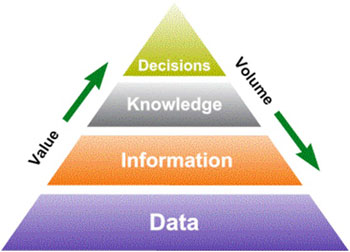
\includegraphics[width=0.7\linewidth]{immagini/datamining}
\caption[Modello del data mining]{Rappresentazione data mining}
\label{fig:datamining}
\end{figure}

Le tecniche maggiormente utilizzate, in questo ambito,
sono: \textit{clustering}, reti neurali, alberi di decisione ed
analisi delle associazioni. Ciascuna comprende un
vasto insieme di metodi e di algoritmi che hanno
l'obiettivo comune di fare emergere \textit{patterns} (sequenze
ripetute, omogeneità, regole, …) dai dati, che, utilizzati
a scopo descrittivo e/o previsivo, costituiscono un
valido strumento di supporto alle decisioni. 


%\epigraph{Citazione}{Autore della citazione}



\chapter{Reactive Programming}
Un sistema reattivo è un sistema \textit{event-driven} che interagisce continuamente con l'ambiente reagendo agli stimoli che da esso gli pervengono.\\
Si assume che i sistemi reattivi:
\begin{itemize}
	\item eseguono con una velocità mai sopraffatta da quella dell'ambiente;
	\item usualmente non terminino mai e quindi siano facilmente caratterizzabili da semplici funzioni che partendo da uno stato iniziale li portino ad uno stato finale.
\end{itemize}
I principi su cui si basa la \textit{reactive programming} sono i seguenti:
\begin{itemize}
	\item \textbf{Responsive:} il sistema deve rispondere ad una richiesta nel minor tempo possibile. Inoltre, con \textit{responsive} si intende anche individuare in maniera rapida un problema e trattarlo in modo efficace;
	\item \textbf{Resilient:} il sistema deve essere \textit{responsive} anche di fronte ad un errore. Ogni sistema non \textit{resilient} è anche non \textit{responsive} nel gestire gli errori;
	\item \textbf{Elastic:} il sistema deve restare \textit{responsive} anche all'aumentare del carico di lavoro. Questo implica che il sistema deve essere scalabile di fronte all'aumento della richiesta senza alcun cambiamento a livello di design del sistema;
	\item \textbf{Message-Driven:} i sistemi \textit{reactive} seguono il modello di programmazione asincrona, ottimizzando l'utilizzando delle proprie risorse.
\end{itemize}
\begin{figure}[h]
\centering
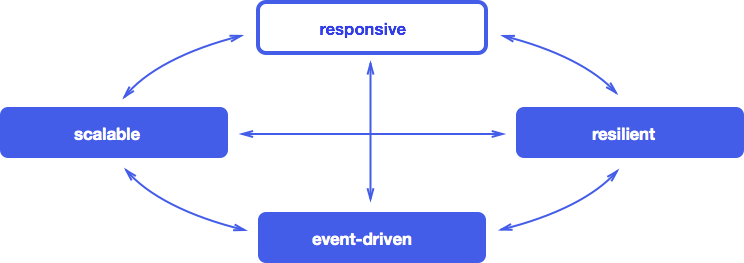
\includegraphics[width=0.7\linewidth]{immagini/react}
\caption[Rappresentazione del modello Reactive Programming]{Rappresentazione del modello Reactive Programming}
\label{fig:react}
\end{figure}




